%%%%% LAS SIGUIENTES OPCIONES SE PUEDEN MODIFICAR DEPENDIENDO DEL FORMATO DESEADO PARA TU DIAPOSITIVA (Comentar o descomentar las líneas correspondientes)


%%%%% Recuerda que usando CTRL + '/' puedes comentar y descomentar rápidamente una línea en LaTeX

%%%%%%%%%%%%%%%%%%%% FORMATO DE ASPECTO %%%%%%%%%%%%%%%%%%%%%%%%%

%%%%%%%%%% ¡IMPORTANTE, ELIGE UN FORMATO DE ASPECTO ANTES DE EMPEZAR TUS DIAPOSITIVAS!
%%%%%%%%%% CAMBIAR EL FORMATO DE ASPECTO UNA VEZ HECHAS LAS DIAPOSITIVAS PUEDE RESULTAR EN QUE TABLAS O ECUACIONES MUY LARGAS NO QUEPAN EN UN SOLO FRAME

% \documentclass[aspectratio = 43]{beamer}  % Formato de aspecto para cañón
\documentclass[aspectratio=169]{beamer} % Formato de aspecto para monitor HD

%%%%%%%%%%%%%%%%%%%% COLORES DE LA DIAPOSITIVA %%%%%%%%%%%%%%%%%%%%%%%%%

% Puedes añadir tus propios colores, sustituye las siguientes líneas por el color deseado en formato RGB

% Color verde
\definecolor{beamer_color}{RGB}{28, 148, 40}
\definecolor{backframe_color}{RGB}{224, 255, 227}


%
% Color violeta
%\definecolor{beamer_color}{RGB}{201, 15, 247}
%\definecolor{beamer_color}{rgb}{0.6, 0.4, 0.8}
%\definecolor{backframe_color}{RGB}{0.6, 0.4, 0.8}


%%%%%%%%%%%%%%%%%%%% FUENTE DEL TEXTO Y LAS ECUACIONES %%%%%%%%%%%%%%%%%%%%%%%%%

% Opción 1. Fuente sans serif tanto en texto como ecuaciones: Deja como comentario todo en las opciones 2 y 3.
% Opción 2. Fuente sans serif en el texto. Fuente serif en las ecuaciones: Descomenta la siguiente línea de texto.
\usefonttheme{professionalfonts}
% Opción 3. Fuente serif tanto en texto como ecuaciones: Descomenta las siguientes líneas de texto.
% \usefonttheme{serif}
% \usepackage[charter, cal = cmcal]{mathdesign}

%%%%%%%%%%%%%%%%%%%%%%%%%%%%%%%%%%%%%%%%%%%%%%%%%%%%%%%%%%%%%%%%%%%%%%%%%%%%%%%%%%%%%%%%%%%%


\usepackage[spanish,mexico,es-noindentfirst]{babel}
\usepackage[utf8]{inputenc}
\usepackage{siunitx}
\usepackage{booktabs}
\usepackage{xcolor}
\usepackage{xspace}
\usepackage{multirow}
\usepackage{graphicx}
\usepackage{lipsum}
\usepackage{tikz}
\usepackage{subcaption}
\usepackage[charter]{mathdesign}
\usepackage{tcolorbox}
\usepackage{caption}
\usepackage{hyperref}

\usetheme{Madrid}

\tcbset{colback=backframe_color, colframe=beamer_color}

\setbeamertemplate{frametitle}{
  \begin{beamercolorbox}[wd=\paperwidth,ht=1cm, sep=0.25cm]{frametitle}
    \begin{tikzpicture}[remember picture,overlay]
      \node[anchor=north east] at (current page.north east) {
\includegraphics[height=0.75cm]{special_figures/TULIX_sinfondo_white}};
    \end{tikzpicture}
    \usebeamerfont{frametitle}\bfseries\insertframetitle
  \end{beamercolorbox}
}

\setbeamertemplate{caption}[numbered]
\setbeamercolor{frametitle}{bg=beamer_color,fg=white}
\setbeamercolor{author in head/foot}{bg=beamer_color,fg=white}
\setbeamercolor{title in head/foot}{bg=beamer_color,fg=white}
\setbeamercolor{date in head/foot}{bg=beamer_color,fg=white}
\setbeamercolor{titlelike}{parent=structure,bg=beamer_color,fg=white}
\setbeamertemplate{section in toc}[sections numbered]
\setbeamertemplate{subsection in toc}[subsections numbered]
\setbeamerfont{section in toc}{series=\bfseries}
\setbeamercolor{section in toc}{fg=black}
\setbeamercolor{caption name}{fg=blue}
\setbeamerfont{caption name}{series=\bfseries}
\setbeamerfont{caption}{size=\small}
\setbeamercolor{bibliography entry author}{fg=black}
\setbeamercolor{bibliography entry title}{fg=black} 
\setbeamertemplate{section in toc}{\inserttocsectionnumber.~\inserttocsection\par}
\setbeamertemplate{subsection in toc}{\hspace{1.5em}\inserttocsectionnumber.\inserttocsubsectionnumber~\inserttocsubsection\par}


\renewcommand{\maketitle}{
\vspace{0.5\baselineskip}

\begin{center}
    
\includegraphics[height=1.25cm]{special_figures/TecNM.jpg}\hfill
    
\includegraphics[height=1.25cm]{special_figures/ITTG.png}\hfill
    
\includegraphics[height=1.25cm]{special_figures/Turix.png}\hfill
\end{center}

\begin{center}
    \textbf{MAESTRÍA EN CIENCIAS EN INGENERÍA MECATRÓNICA}
\end{center}

\titlepage
\vspace{\baselineskip}
\begin{center}
    \small
    \vspace{-2.5\baselineskip}
    Director(es) de la Tesis: Nombre(s) de director(es) de la tesis\\
    Revisor 1: Nombre del primer revisor\\
    Revisor 2: Nombre del segundo revisor\\
\end{center}
}

% \AtBeginSection[ ]
% {
% \begin{frame}{Contenido de la presentación}
% \tableofcontents[currentsection,subsectionstyle = shaded]
% \end{frame}
% }

% \AtBeginSubsection[ ]
% {
% \begin{frame}{Contenido de la presentación}
% \tableofcontents[currentsection,currentsubsection]
% \end{frame}
% } % Si necesitas paquetes adicionales, añadelos al comienzo del documento setup.tex


\title[\textbf{Título de la tesis}]{\textbf{Título de la tesis}}
\author[\textbf{Nombre del tesista}]{\textbf{Nombre del tesista \\ micorreoelectronico@tuxtla.tecnm.mx}}
\date{\textbf{Mes, Año}}




\begin{document}

\begin{frame}
    \maketitle
\end{frame}

\begin{frame}{Contenido de la presentación}
    \tableofcontents
\end{frame}

\section{Cómo usar el formato de diapositivas Turix}

\subsection{Texto}

\begin{frame}{Formatear texto}

\textit{Esto es texto en cursivas.} \textbf{Esto es texto en negritas.} \texttt{Esto es texto en letra de máquina de escribir.}

\tiny{Esto es texto diminuto.}
\scriptsize{Esto es texto muy pequeño.}
\footnotesize{Este texto tiene tamaño para notas al pie.}
\small{Este texto es ligeramente más pequeño al normal.}
\normalsize{Este texto tiene tamaño normal.}
\large{Este texto es ligeramente más grande al normal.}
\Large{Este texto es grande.}
\LARGE{Este texto es aún más grande.}
\huge{Este texto es enorme.}
\Huge{Este es el mayor tamaño posible.}

\end{frame}

\subsection{Cuadros de texto}

\begin{frame}{Insertar cuadros de texto}
    \begin{tcolorbox}[colback=backframe_color,colframe=beamer_color,title=Este es el título del cuadro de texto]
    Esto es un cuadro de texto con título
    \end{tcolorbox}

    \begin{tcolorbox}[colback=backframe_color,colframe=beamer_color]
    Esto es un cuadro de texto sin título
    \end{tcolorbox}
\end{frame}

\subsection{Listas}

\begin{frame}{Insertar una lista}

Esto es una lista ennumerada
\begin{enumerate}
    \item Este es el primer elemento ennumerado.
    \item Este es el segundo elemento ennumerado.
    \item Este es el tercer elemento ennumerado.
\end{enumerate}

Esto es una lista sin ennumerar
\begin{itemize}
    \item Este es el primer elemento.
    \item Este es el segundo elemento.
    \item Este es el tercer elemento.
\end{itemize}
    
\end{frame}

\subsection{Figuras}

\begin{frame}{Insertar figuras}
    Carga tus imágenes a la carpeta \texttt{figuras}. Las imágenes de la carpeta \texttt{special figures} sirven para el formato de la diapositiva.    

    La Figura \ref{fig:red_ramificada} muestra un ejemplo de cómo insertar y referenciar imágenes.

    \begin{figure}[htbp]
        \centering
        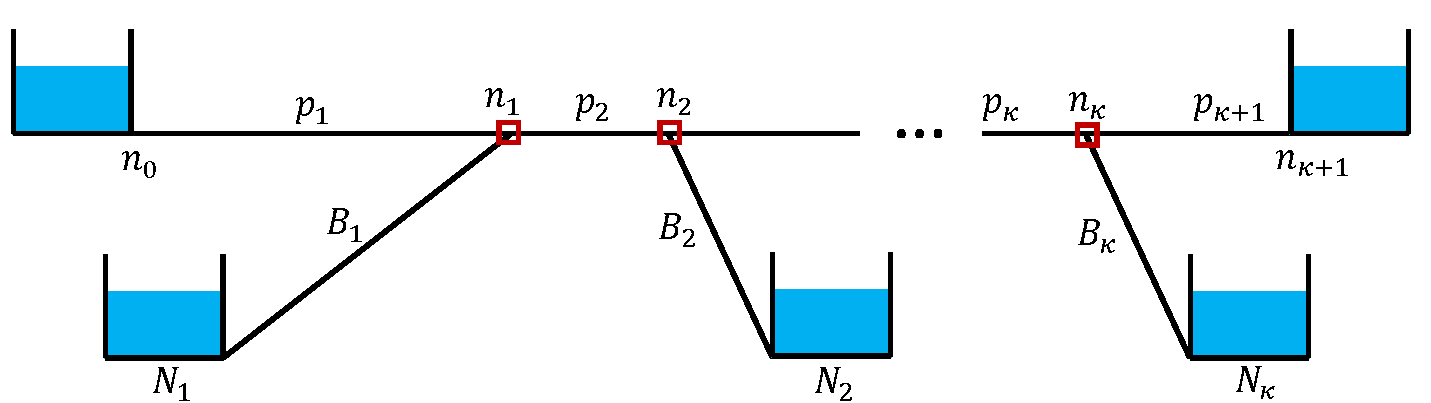
\includegraphics[width = \textwidth]{figuras/BranchedScheme.pdf} % Usar tu propio archivo de imagen. Redimensionar de ser necesario
        \caption{Red con $k$ ramificaciones.} % Usar tu propia descripción
        \label{fig:red_ramificada} % Usar tu propia etiqueta
    \end{figure}
\end{frame}

\begin{frame}{Insertar figuras lado a lado}

    La Figura \ref{fig:comparacion_redes} muestra cómo insertar dos figuras lado a lado.

    \begin{figure}[htbp]
    \centering
    \begin{subfigure}[b]{0.48\textwidth}
        \centering
        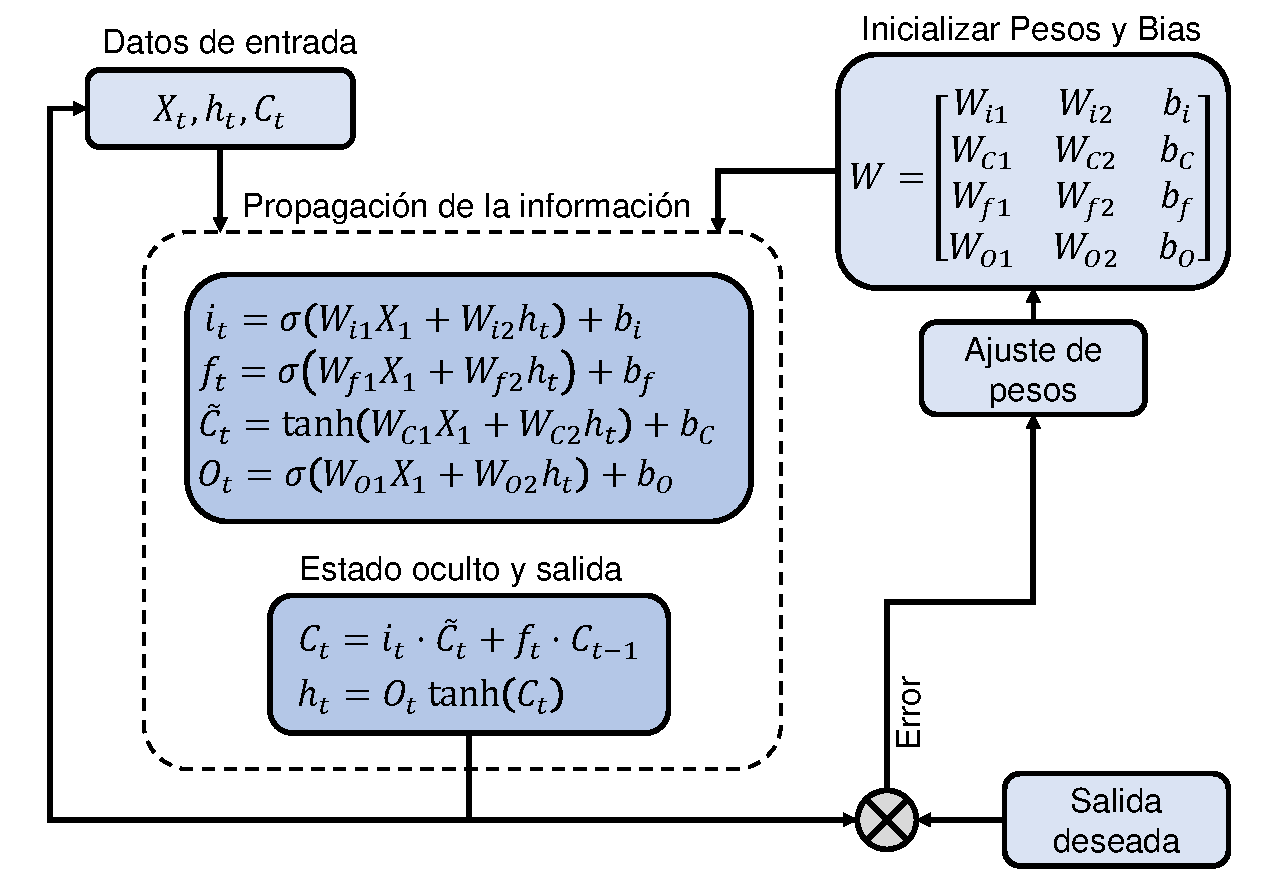
\includegraphics[width=\textwidth]{figuras/LSTM.pdf}
        \caption{Red LSTM}
        \label{fig:figura1a}
    \end{subfigure}
    \hfill
    \begin{subfigure}[b]{0.48\textwidth}
        \centering
        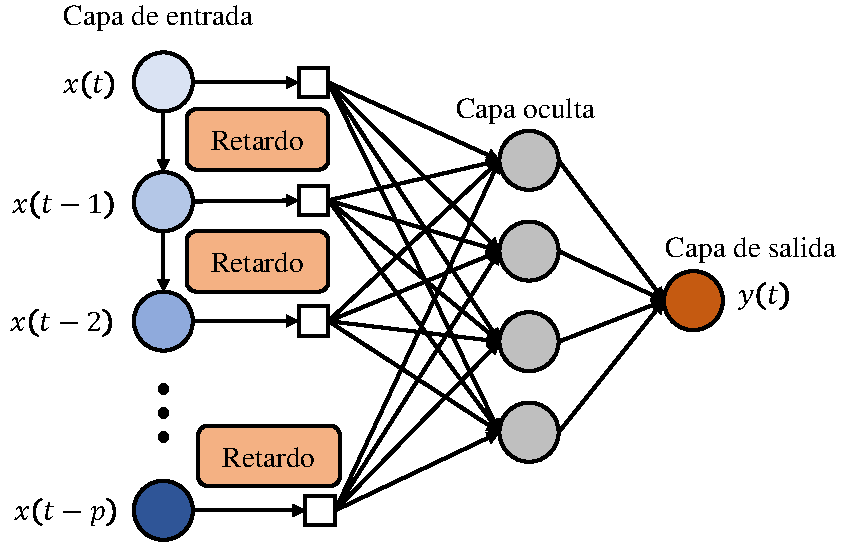
\includegraphics[width=\textwidth]{figuras/TDNN.pdf}
        \caption{Red TDNN}
        \label{fig:figura1b}
    \end{subfigure}
    \caption[Comparación entre dos redes neuronales]{Comparación entre dos redes neuronales}
    \label{fig:comparacion_redes}
\end{figure}
    
\end{frame}


\subsection{Ecuaciones}

\begin{frame}{Insertar ecuaciones}
    Ejemplo de una ecuación numerada:
    \begin{equation}
        \frac{\partial Q\left(z_k,t\right)}{\partial t}+gA_k\frac{\partial H\left(z_k,t\right)}{\partial z_k}+\mu_kQ\left(z_k,t\right)\left|Q\left(z_k,t\right)\right|+g\sin{a_k}=0,
        \label{eq:momentum}
    \end{equation}
    Una ecuación numerada se referencía en el texto usando su \textit{label}: La Ecuación \eqref{eq:momentum} se conoce como la Ecuación del Momentum.
    
    Ejemplo de una ecuación sin numerar:
    $$\frac{\partial H\left(z_k,t\right)}{\partial t}+\frac{b_k^2}{gA_k}\frac{\partial Q\left(z_k,t\right)}{\partial z_k}=0.$$

    Esto es un ejemplo de una ecuación en el texto: $\mu_k=\frac{fQ_k}{2D_kA_k}$  
\end{frame}


\subsection{Tablas}

\begin{frame}{Insertar una tabla}
    La Tabla \ref{tab:ModelosPerdida} muestra un ejemplo de cómo insertar una Tabla de una sola columna. Las tablas requieren la \texttt{caption} en la parte superior
    
    \begin{table}[htbp]
        \centering
        \caption{Fórmulas para el cálculo de las pérdidas de carga en tuberías.}
        \label{tab:ModelosPerdida}
        \small
        \begin{tabular}{ccc}
            \toprule
            \textbf{Modelo de pérdida} & \textbf{Coeficiente} $C$ & \textbf{Exponente} $\sigma$ \\
            \midrule
            Hazen-Williams & $4.727 \mathscr{H}^{-1.852}D^{-4.871}L$ & 1.852 \\
            Darcy-Weisbach & $0.0252f(\varepsilon, D, Q)D^{-5}L$ & 2 \\
            Chezy-Manning & $4.66n^2D^{-5.33}L$ & 2 \\
            \bottomrule
        \end{tabular}
    \end{table}
\end{frame}

\begin{frame}{Insertar tablas a doble columna}

    La Tabla \ref{Tab:Accesorios} muestra un ejemplo de una tabla a dos columnas.
    
    \begin{table}[htbp]
        \centering
        \caption{Accesorios en cada segmento de tubería.}
        \label{Tab:Accesorios}
        \null\hfill
        \footnotesize
        \begin{tabular}{cl}
            \toprule
            \textbf{Nodos inicial y final} & \textbf{Accesorios} \\
            \midrule
            $\text{N}_{1}-\text{N}_{2}$ & 2 Codos 90°\\
            $\text{N}_{2}-\text{N}_{3}$ & 4 Codos 90° \\ 
            $\text{N}_{4}-\text{N}_{5}$ & 2 Codos 90° \\ 
            $\text{N}_{5}-\text{N}_{6}$ & 4 Codos 90° \\ 
            $\text{N}_{7}-\text{N}_{8}$ & 2 Codos 90° \\
            $\text{N}_{8}-\text{N}_{9}$ & 4 Codos 90° \\ 
            \bottomrule
            \end{tabular}
            \hfill\hfill
            \begin{tabular}{cl}
            \toprule
            \textbf{Nodos inicial y final} & \textbf{Accesorios} \\
            \midrule
            $\text{N}_{4}-\text{N}_{10}$ & 1 Codo 90°, 1 Valvula, 1 T \\ 
            $\text{N}_{11}-\text{N}_{12}$ & 4 Codos 90° \\ 
            $\text{N}_{12}-\text{N}_{13}$ & 2 Codos 90° \\ 
            $\text{N}_{6}-\text{N}_{14}$ & 1 Codo 90°, 1 Valvula, 1 T \\        
            $\text{N}_{15}-\text{N}_{16}$ & 2 Codos 90° \\ 
            $\text{N}_{16}-\text{N}_{17}$ & 4 Codos 90° \\ 
            \bottomrule
        \end{tabular}
        \hfill\null
    \end{table}
    
\end{frame}


\section{Referencias}

\begin{frame}{Citas bibliográficas}
    Añade tus referencias en el documento \texttt{biblio.bib} en formato \texttt{BibTex}.

    Esto es una cita de una sola referencia \cite{zhang2017digital}.
    Se pueden citar dos o más referencias en una sola cita separándolas con comas \cite{praks2018advanced,santos2018online}.
    Las referencias se añaden automáticamente en la bibliografía.
\end{frame}

\begin{frame}[allowframebreaks]{Bibliografía}
\bibliographystyle{ieeetr}
\bibliography{biblio}
\end{frame}



\begin{frame}
    \maketitle
\end{frame}


\end{document}